\documentclass[12pt]{article}
%\usepackage{amsmath}
\usepackage{graphicx}
%\usepackage{enumerate}
\usepackage{natbib} %comment out if you do not have the package
\usepackage{url} % not crucial - just used below for the URL 
\usepackage{amsmath, amssymb}


%\pdfminorversion=4
% NOTE: To produce blinded version, replace "0" with "1" below.
\newcommand{\blind}{0}

% DON'T change margins - should be 1 inch all around.
\addtolength{\oddsidemargin}{-.5in}%
\addtolength{\evensidemargin}{-.5in}%
\addtolength{\textwidth}{1in}%
\addtolength{\textheight}{1.3in}%
\addtolength{\topmargin}{-.8in}%


\begin{document}

%\bibliographystyle{natbib}

\def\spacingset#1{\renewcommand{\baselinestretch}%
{#1}\small\normalsize} \spacingset{1}


%%%%%%%%%%%%%%%%%%%%%%%%%%%%%%%%%%%%%%%%%%%%%%%%%%%%%%%%%%%%%%%%%%%%%%%%%%%%%%

\if0\blind
{
  \title{\bf Coupling material and mechanical design processes via computer model calibration}
  \author{Carl Ehrett\thanks{
    The authors gratefully acknowledge \textit{please remember to list all relevant funding sources in the unblinded version}}\hspace{.2cm}\\
    School of Mathematical and Statistical Sciences, Clemson University,\\
    D. Andrew Brown \\
    School of Mathematical and Statistical Sciences, Clemson University,\\
    Evan Chodora \\
    Department of Mechanical Engineering, Clemson University,\\
    Mingzhe Jiang \\
    Department of Chemical and Biomolecular Engineering, Clemson University,\\
    Christopher Kitchens \\
    Department of Chemical and Biomolecular Engineering, Clemson University,\\
    and \\
    Sez Atamturktur \\
    Department of Architectural Engineering, Pennsylvania State University\\}
  \maketitle
} \fi

\if1\blind
{
  \bigskip
  \bigskip
  \bigskip
  \begin{center}
    {\LARGE\bf Title}
\end{center}
  \medskip
} \fi

\bigskip
\begin{abstract}
In traditional engineering design, material selection consists of choosing from a database of known materials, often as a matter of ad-hoc satisficing. 
%
Material design usually occurs separately, without an eye toward specific end-uses.
%
We wed these design processes, designing a material by modeling its performance in a particular application. 
%
We show that techniques for model calibration can be reconceptualized as a method for optimization and applied to solve this material design problem. 
%
We demonstrate our proposed approach by calibrating material design settings to performance targets for a wind turbine blade and by estimating the system's Pareto front with quantified uncertainties. 
\end{abstract}

\noindent%
{\it Keywords:}  Gaussian processes, material design, optimization, Pareto optimality, Uncertainty quantification, wind turbines
\vfill

\newpage
\spacingset{2} % DON'T change the spacing!
\section{Introduction}
\label{introduction}

Real-world optimization problems typically involve multiple objectives. 
%
This is particularly true in the design of engineering systems, where multiple performance outcomes are balanced against budgetary constraints. 
%
Among the complexities involved in optimizing over multiple objectives is the effect of uncertainties in various aspects of the problem. 
%
Design is guided by models known to be imperfect, systems are built using materials with uncertainty regarding their material properties, variations occur in the construction of designed systems, and so on. 
%
These imperfections, uncertainties and errors cause there to be uncertainty also in the solution to a given design problem. 

In traditional engineering design, one designs a system after choosing a material with appropriate properties for the project from a general use database of known materials. 
%
These materials are themselves developed without a specific end-use in mind.
%
As a result, the design of the system is constrained by the initial material selection.
%
By coupling material design and engineering system design, we can combine these two traditionally separate design processes under the umbrella of a unified multiple objective optimization problem.


In this paper, we cast the design problem in the framework of computer model calibration.
%
In traditional calibration, one aligns the computer model output to observations of the real system by estimating unknown parameters in the model.
%
Here, we instead align the computer model to performance and cost targets by finding design variables that optimize the model output with respect to those targets.
%
In addition to optimizing to a specific set of targets, in many situations it is helpful to have a comprehensive picture of optimal outcomes without committing to specific targets.
%
For example, in a system in which there is a trade-off between cost and performance, which region of the model range is considered desirable will depend upon the budgetary constraints of the project.
%
Decision-makers in such a scenario are well-served by having a complete picture of the curve describing the optimal performance at any budget.
%
More generally, in a system with multiple outputs, one wants to estimate the Pareto front of the model range; i.e., the set of points in the model range that are {\em Pareto optimal}.
%
A point is Pareto optimal if and only if, in order to improve any one of its elements, some other element must be made worse off.
%
For example, if a bivariate system in a minimization problem has exactly three output points $a=(2,0)$, $b=(2,1)$, and $c=(1,10)$ then $a$ and $c$ are each Pareto optimal, but $b$ is not, since there is a point (namely $a$) that is less than or equal to $b$ in every output and strictly less than $b$ in at least one output.
%
We show that our proposed methodology can be used to estimate the Pareto front of a system with uncertainty quantification. 
%

Our proposed methodology uses the Bayesian framework first established as a means for computer model calibration by \cite{Kennedy2001}.
% 
This area is furthered by \cite{Higdon2004}, who undertake model calibration with quantification of the related uncertainty. 
They explicitly incorporate uncertainty regarding the computer model input, the bias of the computer model, and uncertainty due to observation error. 
%
The approach of \cite{Higdon2004} is further refined and exemplified by \cite{Williams2006}.
%
\cite{Loeppky2006} offer a maximum-likelihood-based alternative to the Bayesian approach advocated by Kennedy and O'Hagan, intending thereby to improve the identifiability of the calibration parameters in the face of model discrepancy. 
%
\cite{Bayarri2007} extend the approach of Kennedy and O'Hagan, allowing for simultaneous validation and calibration of a computer model (using the same training data). 
%
\cite{Bayarri} apply this methodology to functional data using a hierarchical framework for the coefficients of a wavelet representation. 
%
Similarly, \cite{Paulo2012} apply the approach of \cite{Bayarri2007} to computer models with multivariate output.
%
\cite{Brynjarsdottir2014} demonstrate the importance of strong priors on the model discrepancy term when undertaking calibration.
%

%
Common to those approaches is the conception of calibration as using real observations to get a posterior distribution on unknown parameters $\boldsymbol\theta$ such that the posterior predictive distribution of the model approximates the real system.
%
By contrast, in our proposed methodology, we use artificial observations (representing our design goals) to get a posterior distribution on design variables $\boldsymbol\theta$ such that the posterior predictive distribution of the model approximates our design goals.
%
We describe how, with little added computational cost, the methodology provides an initial rough estimate of the Pareto front for the system, which can be used to select artificial observations that promote strong Bayesian learning about the optimal settings for the design variables $\boldsymbol\theta$.
%
Repeated applications of the procedure can then be used to produce a more thorough estimate of the Pareto front with quantified uncertainties.
%

%
We apply our proposed methodology both to an artificial example and to the problem of finding material design settings to optimize the performance and cost of a wind turbine blade of fixed outer geometry.
%
The wind turbine blade in question is to be constructed using a composite material.
%
One design variable targeted for optimization is the \emph{volume fraction}, which is the ratio of the \emph{filler} to \emph{matrix} used in the composite material.
%
In a composite, the matrix holds the filler together; an example would be concrete, in which a filler of loose stones is combined with a matrix of cement.
%
Another design variable is the thickness (in mm) of the shear web used in the blade.
%
Our material design goal is to reduce the cost per square meter of the composite material, the rotation (in radians) of the blade when under load, and the deflection (in meters) of the blade tip when under load.
%

%
In Section \ref{calib_for_design}, we review the calibration framework that serves as the basis for our proposed design optimization approach. 
%
In Sections \ref{example} and \ref{application}, we apply our proposed methodology to the example involving simulated data and to wind turbine blade design.
%
In Section \ref{application}, we show how our approach can be used to produce an estimate of the Pareto front of the wind turbine blade system while quantifying associated uncertainty.
%
Section \ref{conclusion} concludes with discussion of the results and thoughts about future directions.

%
\section{Calibration for design}\label{calib_for_design}
%\subsection{Calibration framework} \label{calib_framework}

%
\subsection{Gaussian process emulators for calibration}
%
In this work, when an emulator is needed we assume the use of a Gaussian process (GP) emulator.
%
Just as a multivariate Gaussian random variable is characterized by its mean vector and covariance matrix, a Gaussian process is fully characterized by its mean function $\mu:D\to \mathbb R$ and covariance function $C:D\times D\to \mathbb R$, where $D$ is the domain of the process. 
%
Thus for any points $\mathbf x,\mathbf y$ in the domain of the Gaussian process, $\mu(\mathbf x)$ gives the mean of the Gaussian process at $\mathbf x$, and $C(\mathbf x, \mathbf y)$ gives the covariance between the values of the Gaussian process at points $\mathbf x$ and $\mathbf y$.
%
The distribution of the process at any finite number of points is multivariate Gaussian with mean vector and covariance matrix determined by $\mu(\cdot)$ and $C(\cdot,\cdot)$.
%
In principle, model calibration need not rely on a GP emulator, or any other sort of emulator; one could (e.g.) complete a full Bayesian analysis via Markov chain Monte Carlo \citep[MCMC;][]{Gelfand1990} by running the relevant computer model at each iteration of the chain. 
%
%\cite{Hemez2011} compare the use of Kennedy-O'Hagan-style calibration with and without an emulator. 
%%
In Section \ref{example} we assume fast-running computer code for the simulated example.
%
However, computer models are frequently too computationally expensive to allow for such expenditure. \citep{VanBuren2013,VanBuren2014}.
%
Instead, a computationally tractable emulator can be constructed using a sample of output from the computer model. 
%

%
GPs are popular prior distributions on computer model output for three reasons.
%
Firstly, because their use does not require detailed foreknowledge of the model function's parametric form. 
%
Secondly, GPs easily interpolate the computer model output, which is attractive when the computer model is deterministic and hence free of measurement error. 
%
This is usually the case, although some attention in model calibration \citep[e.g.,][]{Pratola2018} has focused specifically on stochastic computer models. 
%
Thirdly, GPs facilitate uncertainty quantification through the variance of the posterior GP. 
%
This section provides brief background on Gaussian processes and their use in regression broadly, and in computer model calibration specifically.
%

%
The use of GPs to produce a computationally efficient predictor of expensive computer code given observations of code output at $\mathbf X=(\mathbf x_1,\ldots,\mathbf x_n)^T$ is advocated by \cite{Sacks1989} and explored at length by \cite{Santner2003a}.
%
Since computer code is typically deterministic, these applications differ from the focus of \cite{OHagan1978} in that the updated GP is induced to interpolate the computer output $\boldsymbol \eta = (\eta(\mathbf x_1),\cdots,\eta(\mathbf x_n))^T$. 
%
\cite{Kennedy2001} use GPs for computer model calibration. 
%
\cite{Kennedy2006} showcase this use of GP emulators for uncertainty and sensitivity analyses. 
%
\cite{Bastos2009} describe both numerical and graphical diagnostic techniques for assessing when a GP emulator of a computer model is successful, as well as discussion of likely causes of poor diagnostic results. 
%
While most work in the area of GP emulation uses stationary covariance functions 
%(in which $\mu(\cdot)$ is constant and $C(\mathbf x,\mathbf x' )\equiv C(\mathbf x-\mathbf x' )$ depends only on the difference between $\mathbf x$ and $\mathbf x'$, rather than on their location in the input domain) 
and quantitative inputs, efforts have been made to branch away from these core assumptions. 
%
\cite{Gramacy2008} use treed partitioning to deal with a nonstationary computer model. 
%
\cite{Qian2008} explore methods for using GP emulators that include both quantitative and qualitative inputs.
%

%
Whether or not an emulator is used, in the framework implemented here one may consider a computer model to be of the form $\eta(\mathbf x,\boldsymbol \theta)$, where $(\mathbf x,\boldsymbol \theta)$ comprise all inputs to the model. 
%
The vector $\boldsymbol \theta$ denotes the collection of design variables. 
%
The vector $\mathbf x$ is the collection of all other inputs that are known and/or under the control of the researcher.
%
We call $\mathbf x$ the \emph{control inputs}.
%
Thus, the model is
%
\begin{equation} \label{eq:model_gen}
y(\mathbf x)=\eta(\mathbf x,\boldsymbol \theta) + \delta(\mathbf x)+\epsilon(\mathbf x),
\end{equation} 
%
where $y(\mathbf x)$ describes a model outcome at control inputs $\mathbf x$, $\delta(\cdot)$ describes the model discrepancy (the systematic bias of the model as an estimate of the response) and $\epsilon(\cdot)$ is a mean-zero error, often assumed to be i.i.d.\ Gaussian. 
%

%
To employ an emulator, suppose that we have inputs $\{(\mathbf x_i,\mathbf t_i)\}_{i=1}^n\subseteq \mathbb R^p\times \mathbb R^q$ scaled to the Cartesian product of the $p-$ and $q-$dimensional unit hypercubes, and that we have completed computer model runs 
%
$\eta\left(\mathbf x_i,\mathbf t_i\right)$ for $i=1,\cdots,n.$
%
Define the GP prior for modeling $\eta(\cdot,\cdot)$ as follows. 
%
Let the mean function $\mu(\mathbf x,\mathbf t)=c$, $c$ a constant. 
%
Set the covariance function in terms of the marginal precision $\lambda_\eta$ and a product power exponential correlation function:
%
\begin{equation}\label{eq:Hig_cov}
C((\mathbf x,\mathbf t),(\mathbf x',\mathbf t')) = \frac 1\lambda_\eta \prod_{k=1}^{p}
\exp \left(-\beta^\eta_k|x_k-x_k'|^{\alpha_\eta}\right) \times
\prod_{j=1}^{q}
\exp \left(-\beta^\eta_{p+j}|t_j-t_j'|^{\alpha_\eta}\right)
\end{equation}
%
where each $\beta_k$ describes the strength of the GP's dependence on one of the elements of the input vectors $\mathbf x$ and $\mathbf t$, and $\alpha_\eta$ determines the smoothness of the GP. 
%
The model is completed by specifying priors for the hyperparameters $c,\lambda_\eta,\alpha_\eta,$ and $\beta^\eta_j$ for $j=1,\ldots,p+q$, though in practice these are often set to predetermined values.
%

%
\subsection{Design to target outcomes}
%

%
Call design goals (such as performance and cost targets) treated as observations in the proposed design procedure ``target outcomes'', and call the proposed procedure, which uses a Bayesian model calibration framework with target outcomes in place of real observations, ``calibration to target outcomes" (CTO). 
%
Thus target outcomes are a sort of artificial data, and the calibration procedure is carried out as if these artificial data had been observed in reality.
%
Just as in traditional calibration, in which the result of the procedure is a distribution on the calibrated parameter $\boldsymbol\theta$ to approximate the observed data, in CTO the result is a distribution on the design parameter $\boldsymbol\theta$ which induces the model to approximate the performance and cost targets.
%
The posterior predictive distribution is thereby pushed toward the target outcomes.
%
%Of course, computer models are more malleable than reality, and it is trivial to modify a computer model so that its output matches any given target. 
%
The model used is assumed to yield accurate results within the design domain.
%
Future work in this area will address the case of models that are known or suspected to suffer from systematic bias.
%

%
%One might worry that calibrating a model to artificial ``target outcomes'' will undermine the model's accuracy, since the model is essentially being fed false data.
%
%It is both easy and pointless to create a model which is a computational ``yes man''. 
%
%In many cases, however, one is fortunate to have (perhaps after undertaking traditional model calibration, validation and verification) a computer model that is known to be faithful to reality over a given set $\mathcal T$ of user specified input settings.
%uniformly valid over a given set $\mathcal T$ of controllable parameters $t$, i.e., the model is known to be faithful to reality over $\mathcal T$. 
%
%In such a circumstance, in searching for $\mathbf t\in\mathcal T$ so that the model output matches one's targets, one does not risk using making predictions at settings under which the model is unreliable. 
%
%Instead, one finds a distribution of the settings that achieve the most realistic approximation to the target outcomes.

The tools of model calibration founded in the work of \cite{Kennedy2001} retain their advantages under our proposed methodology.
%
Most centrally, calibration to target outcomes $\mathbf y$ produces not merely a point estimate $\mathbf t^*\in\mathcal T$, but rather a posterior distribution of $\mathbf t|\mathbf y$ reflective of remaining uncertainty about the appropriate value of $\mathbf t^*$. 
%
Such uncertainty may have its source in parameter uncertainty (uncertainty about the values of model inputs other than the design variables), model form uncertainty (uncertainty about how closely the code approximates reality), and that which traditional calibration would consider observation error. 
%
Of course,  targets are not actually observations, so the concept of observation error does not cleanly transfer. 
%
However, a similar uncertainty would be that due to how close reality \emph{can} come to our target outcomes. 
%
The Bayesian model calibration framework allows for the quantification of all of these uncertainties. 
%
Furthermore, by the use of informative priors on the model discrepancy and observation error, the identifiability concerns of the Kennedy-O'Hagan approach can be mitigated \citep{Bayarri2007,Tuo2016}.

In general, target outcomes should aim only a little beyond what is realistically achievable; only as much as is necessary to ensure the targets are at least as ambitious as any true optimum in the system.
%
Three reasons why one should go only a little beyond that are as follows: 
%
Firstly, if target outcomes are set to be too farfetched, then the procedure can become computationally unstable due  to underflow and round-off error, since any value of $\boldsymbol \theta$ within its support will have extremely low likelihood.
%
Secondly, increasing the distance of the target outcomes from the optimal region reduces the identifiability of that region.
%
CTO finds the region of the parameter space with output closest to the target outcomes.
%
If the entire feasible performance range is far from the target outcomes, then the optimal region will in relative terms be only a little closer than the rest of the model range. 
% 
This is the same effect as when the variance of the observation error is much larger than the variance of the prior distribution on a parameter; i.e., the posterior is much more strongly determined by the prior than the likelihood, resulting in limited Bayesian learning about quantities of interest.
%The nearness of the optimum to another point in the parameter space is relative to the estimated error at the optimum, and therefore if the entire model range is far from the target observations, then all points in the parameter space will be 
%
%relative difference between the distance to the Pareto front and the distance to other regions of the model range, thereby decreasing the identifiability of the region to which one wishes to calibrate.
%
A third reason to keep target outcomes close to the model range is that the targets lose their interpretability when they take on values that are implausible or impossible. 
%

%%
%A third option is also explored in Section \ref{application}'s treatment of the material design application. 
%%
%This option is not truly another means of achieving a calibration target, but rather is simply the decision to refrain from doing so. 
%%

When a target cannot be selected (for example, because priorities regarding cost and performance trade-offs have not yet been settled), design can be carried out using each point in a grid over the region of plausible target values.
%
For instance, one can design to performance targets under each point of a grid of ``known'' costs, rather than designing with a specific desired cost.
%
In doing so, we present a comprehensive picture of optimal parameter distributions and resulting performance under a range of costs, which could inform the process of setting a budget.
%

%
It is common to plug in the MLEs of the GP covariance hyperparameters $\lambda_\eta$ and $\boldsymbol \beta^\eta$ in \eqref{eq:Hig_cov} instead of including them in a full Bayesian analysis \citep{Kennedy2001,Santner2003a,Qian2008,Paulo2012}.
%
In our proposed methodology, that is not merely a convenience, but rather is essential.
%
This is because in a full Bayesian analysis, the posterior distributions of $\lambda_\eta$ and $\boldsymbol\beta^\eta$ would depend upon target outcomes which are not real observations of the system.
%
The resulting emulator would be trained not only on the simulator output, but also on our performance and cost targets, which will typically be (intentionally) unrealistic.
%
As argued by \cite{Liu2009}, it is preferable to avoid training a computer model emulator using data which do not arise from that model.
%
Therefore, we use values found by maximizing the log likelihood of the observations of the simulation with respect to $\lambda_\eta$ and $\boldsymbol\beta^\eta$.
%
We set the GP to have constant mean $c=0$, which works well when (as here) the GP is not used for extrapolation \citep{Bayarri2007}.
%
We set $\alpha_\eta = 2$, which assumes that the model output is infinitely differentiable.

We similarly model the discrepancy term $\delta(\cdot)$ as a GP, also with mean zero, and with covariance function
%
%\begin{equation}
$C_\delta(\mathbf x,\mathbf x') = \lambda_\delta^{-1} \prod_{k=1}^p
\exp\left( -\beta_k^\delta |x_k-x_k'|^{\alpha_\delta} \right).$
%\end{equation}
%
This is included in the model to capture systematic discrepancy between target outcomes and the feasible model range.
%
We use priors
%$\lambda_\delta \sim \mathrm{Gamma}(5,\mathrm{scale}=5)$ and 
$\rho^\delta_k \sim \mathrm{Beta}(1,0.3),$
where $\rho_k^\delta = \exp(-\beta_k^\delta/4)$ for $k=1,\ldots,p$. 
%
A Gamma prior is appropriate for $\lambda_\delta$, with strength determined by the amount of prior information available. 
%
With sufficient prior information, though, we can set $\lambda_\delta$ to be constant. 
%
Details surrounding the choice of prior for $\lambda_\delta$ are discussed below.
%
As with the covariance function of $\eta(\cdot,\cdot)$, we set $\alpha_\delta=2$.

Let $\boldsymbol \eta = (\eta(\mathbf x_1,\mathbf t_1),\cdots,\eta(\mathbf x_n,\mathbf t_n))^T$ be the vector of completed runs of the simulator, $\mathbf y = (y(\mathbf x_{n+1}),\cdots,y(\mathbf x_{n+m}))^T$ the target outcomes we wish to induce the system to achieve, 
and $\mathcal D = (\boldsymbol \eta^T,\mathbf y^T)^T$.
%
Then $\mathcal D | \boldsymbol \theta,\widehat{\lambda_\eta}, \widehat{\boldsymbol \rho^\eta},\lambda_\delta,\boldsymbol \rho^\delta$ is distributed as multivariate normal with mean 0 and covariance $\mathbf C_\mathcal D$, a matrix with $i,j$ entry equal to 
$
C((\mathbf x_i,\mathbf t_i),(\mathbf x_j,\mathbf t_j)) + I(i,j>n)\cdot(C_{obs}(\mathbf x_i,\mathbf x_j) + C_\delta(\mathbf x_i,\mathbf x_j))
$
%where $C_{obs}(\cdot,\cdot)$ is the (known) observation error variance.
%
where $C_{obs}(\cdot,\cdot)$ serves as ``observation error'' of our own target outcomes, since in a typical case one can at best identify a small region within which the choice of any particular point as a target outcome would be arbitrary due to our acceptable tolerance.
%
Thus, $C_{obs}(\mathbf x_i,\mathbf x_j) = \sigma^2\delta^K_{ij}$, where $\delta^K$ is the Kronecker delta and $\sigma^2$ is chosen to reflect the desired tolerance level, such that targets within $\sigma$ of each other are considered to be roughly equivalent.
%
The appropriate setting for $\sigma^2$ will differ across applications.
%
For our applications, we set $\sigma^2=0.05$ (with target outcomes standardized to have mean zero and prior standard deviation 1).
%
Notice also that $C_{obs}(\cdot,\cdot)$ serves to add a nugget to the covariance matrix produced by $C_\delta(\cdot,\cdot)$.
%
Aside from easing matters computationally (by improving the conditioning of the covariance matrix), the addition of such a nugget can improve the quality of the fit of the GP discrepancy $\delta$ \citep{Gramacy2012}.
%
Setting a uniform prior on the design variables $\boldsymbol\theta$, the joint posterior density under the model is
%
\begin{equation} \label{eq:full_dist}
\pi(\boldsymbol \theta,\lambda_\delta,\boldsymbol \rho^\delta|\mathcal D,\widehat{\lambda_\eta},\widehat{\boldsymbol \rho^\eta})
\propto \pi(\mathcal D | \boldsymbol \theta,\widehat{\lambda_\eta}, \widehat{\boldsymbol \rho^\eta},\lambda_\delta,\boldsymbol \rho^\delta) \times %\pi(\lambda_\eta) \times 
%\pi(\boldsymbol \rho^\eta) \times 
\pi(\lambda_\delta) \times \pi(\boldsymbol \rho^\delta).
\end{equation}
%
Markov chain Monte Carlo methods are useful for estimating features of the posterior distribution.

%
In order to successfully locate the optimal design region, it is necessary either to place an informative prior on the marginal precision $\lambda_\delta$ of the discrepancy $\delta(\cdot)$, or else to specify $\lambda_\delta$ outright. 
%
Otherwise, the optimal region of the design variable space will suffer from poor identifiability.
%
This longstanding concern was raised in the discussion of \cite{Kennedy2001}, as well as by \cite{Bayarri2007}, \cite{Tuo2015}, and \cite{Plumlee2017}.
%
How informative one's prior on $\lambda_\delta$ will be depends upon how much one knows about the true Pareto front prior to undertaking CTO.
%
For instance, if in a univariate case it is known with some confidence that the true optimum is nearly constant as a function of the other model inputs, and that it occurs in the interval $[10,11]$, then a constant target outcome of $9$ could be used with an informative prior tailored to this prior knowledge of the approximate resulting discrepancy.
%

Where the prior on $\lambda_\delta$ cannot be chosen to be \emph{accurate} (due to insufficient prior knowledge of the Pareto front) it should be chosen to \emph{overestimate} the precision.
%
Otherwise, underestimation of $\lambda_\delta$ may lead to poor identifiability of the optimal design region by granting the model too much flexibility in systematically deviating from the targets.
%
This is because $\lambda_\delta$ affects the expected distance of the target outcomes from the posterior predictive distribution.
%
Thus, underestimating $\lambda_\delta$ can result in there being little penalty in leaving the region of the model range that is closest to the target outcomes.
%
When setting a prior that overestimates $\lambda_\delta$, the posterior distribution of $\lambda_\delta$ becomes less reliable than when an accurate prior is used.
%
Nonetheless, even when $\lambda_\delta$ must be overestimated, the posterior distribution of $\boldsymbol \theta$ will still peak at the optimal design region, since overestimation of $\lambda_\delta$ forces the mean-zero discrepancy to be small and thereby only increases the penalty of leaving the optimal region.
%
Thus, while relying on vague knowledge of the optimum does interfere with one's ability to estimate the true discrepancy of the model from the target outcomes, one may still locate the posterior mode(s) of $\boldsymbol \theta$ and thereby the optimal settings for the model.
% %HERE
However, if $\lambda_\delta$ is too highly overestimated, then MCMC may become trapped in a local mode, leading to convergence problems. 
%
In short, while the proposed methodology is forgiving of overestimation of $\lambda_\delta$, the identifiability of the optimal design region(s) is best served by supplying as informative of a prior as possible. 

%
In situations where one lacks the prior knowledge necessary to select target outcomes near the Pareto front and an accurate prior for $\lambda_\delta$, an alternative is to use a ``preliminary round'' of CTO to {\em estimate} the Pareto front.
%
For example, consider again the univariate case, supposing now that we know only that the optimal output is approximately constant somewhere in the range $(0,20)$. 
%
One could perform CTO directly with constant target outcome below the known model range (e.g., $-1$) and prior on $\lambda_\delta$ that weakly pulls the posterior predictive distribution toward the lower end of its range (e.g., exponential with rate 2).
%
If the true optimal output turns out to be close to the lower end of its known range, this will likely work well.
%
However, if the optimal output turns out to be sufficiently high, the optimal region of the parameter space could suffer from poor identifiability.
%
To avoid this, one can instead perform CTO still with constant target outcome $-1$ but with a prior on $\lambda_\delta$ that deliberately exploits the identifiability problems of the Kennedy-O'Hagan framework in order to explore large regions of the parameter space -- say, exponential with rate 0.1.
% 
Though the resulting posterior distribution will have greater density in the optimal region(s) than would a uniform sampling, it will likely not center in the optimal region, instead covering a larger area of the model range.
%
The resulting posterior predictive distribution can be filtered to retain only its Pareto front, and this can be used as an estimate of the true Pareto front in the vicinity of the target outcome.
%
%This preliminary estimate (unlike the estimate achieved after full CTO) does not include uncertainty quantification. 
%
The preliminary estimate allows one to select a new set of target outcomes that is known to lie near the optimal region, along with an accurate and informative prior on $\lambda_\delta$ that reflects the estimated distance between the new target and the optimal region.
%
Performing CTO with these new targets and prior will result in a posterior distribution that concentrates on the optimal region, and the resulting posterior predictive distribution will allow one to estimate the optimal output with appropriate quantification of the uncertainty.
%
%
%To continue the above example, preliminary CTO may show that the true optimum across the domain of the control inputs is in the interval $[10,11]$, which puts one in a position to use the aforementioned combination of a constant target outcome of 9 and $\lambda_\delta\sim$ Gamma(20, 20) prior, or even a degenerate prior with $\lambda_\delta$ set equal to 1.
%
The full CTO process, including preliminary estimation of the Pareto front, is given in Algorithm 1.

\begin{figure}
\centering
\begin{tabular}{|l|p{5.5in}|}
\hline
\multicolumn{2}{|c|}{Algorithm 1: Full CTO procedure including preliminary estimation of Pareto front}\\
\hline
1.&Set target outcomes to lie outside of the model range.\\
2.&  Set a vague prior on $\lambda_\delta$.\\
3.&  Perform MCMC and use the resulting posterior samples of $\boldsymbol\theta$ to draw from the posterior predictive distribution of the model output.\\
4.&  Filter the resulting predictions to retain only the Pareto optimal values. The remaining set of values $\mathcal P$ estimates the Pareto front.\\
5.& Select new target outcomes using $\mathcal P$. These may be entirely new targets chosen after examining $\mathcal P$, or may simply be updated automatically to set each target outcome to be the same (small) distance $1/\sqrt{\lambda}$ (for some $\lambda$) from $\mathcal P$.\\
6.& Set a strong (or degenerate) prior on $\lambda_\delta$ with mean $\lambda$.\\
7.& Perform MCMC in the usual way.\\
\hline
\end{tabular}
\label{alg:CDO_alg}
\end{figure}


An illustration of the benefits of preliminary CTO appears in Figure \ref{fig:do_selection_example}.
%
\begin{figure}
\centering
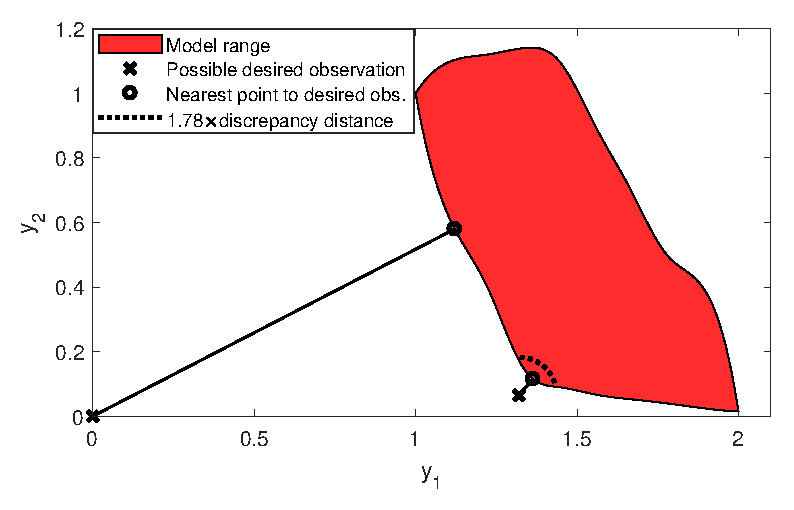
\includegraphics[scale=.8]{FIG_des_obs_selection_example.eps}
%\captionsetup{width=.4\linewidth}
\caption{Two potential choices of target outcomes. 
%
The distance from $(0,0)$ to the farthest point in the model range is only 2 times the distance to the nearest point. 
%
By contrast, for the point (1.32,0.065), the dotted line shows the small region of the model range within 2 times the distance to the nearest point.}
\label{fig:do_selection_example}
\end{figure}
%
Suppose that, prior to undertaking CTO, we know only that the model outputs are positive.
%
Then $(0,0)$ is a natural choice to use as a target outcome.
%
However, in this case, that choice of target outcome will yield three problems.
%
Firstly, the model range is distant from $(0,0)$.
%
As a result, the optimal region is, relative to the size of the model range, not much closer to the target outcome than other regions of the model range.
%
Indeed, the farthest point in the entire model range is only 2 times farther from $(0,0)$ than is the nearest point.
%
This leads to very poor identifiability of the optimal region, since large portions of the model range are roughly as close to $(0,0)$ as is the optimum.
%
Secondly, the optimal region determined by the choice of $(0,0)$ is somewhat arbitrary.
%
Notice that in this example the entire ``left'' and ``bottom''  edges of the model range comprise the Pareto front.
%
The point closest to $(0,0)$ is not intrinsically superior to any other point on the Pareto front.
%
Its uniqueness lies solely in being nearest to the origin, and that choice of target outcome was itself driven merely by our ignorance of the model range.
%
Thirdly, since we don't know the model range, we are not in a position to set an informative prior for $\lambda_\delta$.
%
By contrast, suppose now that we have performed preliminary CTO and have available a rough estimate of the Pareto front, empowering us to choose another point as our target outcome -- for example, the point $(1.32,0.065)$ pictured in Figure \ref{fig:do_selection_example} targets a point of diminishing returns where allowing $y_1$ to increase further leads to diminishing returns in reducing $y_2$.
%
Alternatively, one could select $(1,0.015)$, since this is the minimum of each model output, and thus will optimize to a region minimizing the sum of squared increases in each output over its minimum.
%
Either choice of new target outcome would answer all of the above problems.
%
Firstly, each point is much closer to the model range, leading to greater identifiability.
%
Secondly, these choices of target outcome and resulting optima are not arbitrary, but rather are driven by articulable goals informed by an estimate of the Pareto front.
%
Thirdly, with a rough estimate of the Pareto front we can supply a strong (or even degenerate) prior for $\lambda_\delta$.
%
Note also that when an emulator is used, a preliminary round of CTO can use the same set of model observations as the subsequent CTO for the training points of the emulator.
%
So performing preliminary CTO does not add to the total budget of model runs, and can thus be a computationally cheap supplement to CTO.
%

%
\section{Simulated Example}\label{example}
%

%
As an illustration of our proposed procedure with known solution, consider the following problem of minimizing a function with trivariate output. 
%
Let $(x,\boldsymbol \theta)$ be the vector of inputs, with scalar control input $x\in[1.95,2.05]$ and design variables $\boldsymbol \theta = (\theta_1,\theta_2)\in[0,3]\times[0,6]$.
%
We seek optimal settings for $\boldsymbol\theta$.
%
We consider three outputs:
%
$
y_1 = \left(\theta_1 \exp\left(-\left(\theta_1 + \lvert \theta_2-\frac{\pi x}2\rvert \right)\right)+1\right)^{-1}$, 
$
y_2 = \left(\theta_2^{x-1} \exp\left(-0.75 \theta_2\right) + 1 \right)^{-1}
$, and
$
y_3 = 15 + 2 \theta_1 + {\theta_2^2}/4.
$
%
We suppose that prior to undertaking CTO we know only that the model outputs are positive.
%
Figure \ref{fig:toy_sim_outputs} displays the $y_1, y_2$, and $y_3$ surfaces as functions of $\theta_1$ and $\theta_2$ at $x = 2$.
%
\begin{figure}
\centering
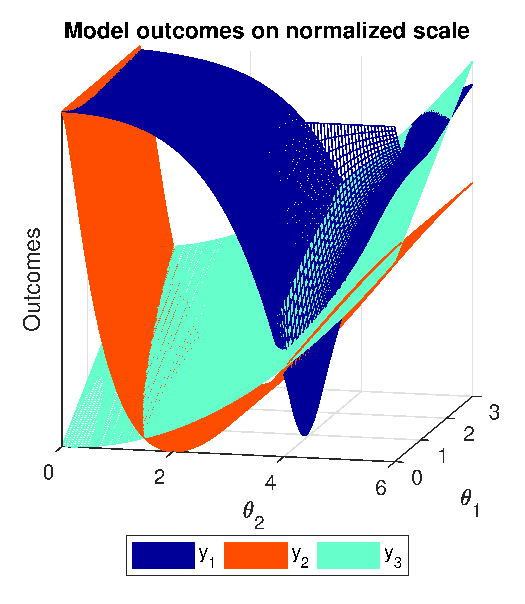
\includegraphics[scale=.8]{FIG_toy_sim_model_outputs.eps}
%\captionsetup{width=.4\linewidth}
\caption{True outputs of the example model.}
\label{fig:toy_sim_outputs}
\end{figure}
%
Assuming an easily evaluated model (so that a GP code surrogate is not needed), we have
%
$
\mathbf z(x) = \mathbf f(x,\boldsymbol \theta) + \delta(x) + \boldsymbol\epsilon
$
%
for target outcome $\mathbf z$, where $\mathbf f = (y_1,y_2,y_3)^T$ is the model output, $\delta(\cdot)$ is the discrepancy between the optimal region and the target outcome, and $\boldsymbol \epsilon$ is the target outcome tolerance and follows a $N(\mathbf 0,0.05I)$ distribution. 
%
%Aside from easing matters computationally, $\boldsymbol \epsilon$ serves as ``observation error'' of our own target outcomes, since in a typical case one can at best identify a small region within which the choice of any particular point as a target outcome would be arbitrary due to our acceptable tolerance.
%

We initially set the target outcomes to $(0,0,0)$, constant as a function of $x$. 
%
We then estimated the Pareto front via a preliminary round of CTO with $\lambda_\delta\sim \mathrm{Exp}(1)$ in order to estimate the standardized distance of the target outcome from the Pareto front.
%
We filtered the resulting posterior predictive distribution to retain only the Pareto optimal points.
%
Rescaling so that each model output $y$ is replaced with $y^*=(y-\mathbb E(y))/\sqrt{\mathbb V(y)}$, the distance from the Pareto front to the target outcome is 16 units.
%
This is large compared to the model range, at roughly four times its diameter.
%
As a result, the use of $(0,0,0)$ as a target outcome would lead to poor identifiability of the optimal region. 
%
This is because the target outcome is approximately the same distance from any point in the model range, relative to the distance from the target outcome to the optimal region.
%
Therefore in order to improve identifiability of the optimal region, we updated the target outcome to lie along the line connecting the original target outcome to the nearest point of the estimated Pareto front, but now closer to the latter.
%
We chose a distance of one unit away, as this is roughly the sample standard deviation of the distances from each model output to the sample mean.
%
We thereby approach the estimated Pareto front closely (relative to the size of the model range) while remaining confident that the new target outcome of $(0.71, 0.71, 17.92)$ still outperforms the true Pareto front.
%
This confidence is based on the observation that $F(\mathbf x-(0.71,0.71,17.92)^T)>0.95$, where $x$ is the nearest point of the estimated Pareto front and $F$ is the cdf of the tolerance $\boldsymbol\epsilon\sim	 N(\mathbf 0, 0.05I)$.
%
We then set the marginal precision of the discrepancy function $\lambda_\delta=1$ for subsequent CTO, corresponding to a degenerate prior informed by the estimated distance of the new target outcome from the Pareto front.
%
%Observation error $\epsilon(\cdot)$ from \eqref{eq:model_gen} was taken to be distributed as $N(0,0.05)$ for all $x$, which ensures that almost all ($>95\%$) of the target outcomes' probability mass is outside our estimate of the Pareto front.
%
For comparison, we also performed CTO directly, without the use of preliminary CTO.
%
To do so, we used our original target outcome of $(0,0,0)$ with a Gamma(10,10) prior deliberately overestimating $\lambda_\delta$.
%
Notice that although the Gamma prior from direct CTO and the degenerate prior $\lambda_\delta=1$ from full CTO have the same means, this is an overestimation only in the case of direct CTO, since the two posterior explorations used different target outcomes.
%
%While the Exp(1) prior used in preliminary CTO does pair a mean of 1 with target outcome (0,0,0), the exponential prior does not penalize low values of $\lambda_\delta$, and so fails to result in overestimation of $\lambda_\delta$.
%
Figure \ref{fig:toy_sim_results} shows the resulting posterior distributions of the two design procedures, including the marginal distributions of the design variables. 
%
The marginals in each case show substantial Bayesian learning compared to the prior (uniform) distribution of the design variables. 
%
CTO successfully maps the contours of the optimal region in each of the two cases, and peaks near the true optimum. 
%
However, the benefits of preliminary CTO are apparent in the greater spread of the posterior distribution from direct CTO.
%
The marginals are much more sharply peaked after using preliminary CTO, with much lighter tails.
%
Thus relying on an estimate of the Pareto front when selecting target outcomes for CTO can greatly reduce uncertainty about the optimal settings for $\boldsymbol\theta$ and for the resulting performance and cost outcomes for the system.
%
%In addition, through preliminary CDO we gained the estimate $\lambda_\delta\approx1$, whereas direct CDO leaves us with no reliable estimate of the marginal precision of the discrepancy.
%
This simulation example illustrates that CTO can be used directly with little foreknowledge of a system's Pareto front, but that greater identifiability of the optimal region can be achieved using preliminary CTO.
%Among the posterior predictive samples $\tilde {\mathbf y}$ associated with each draw of $\boldsymbol \theta$, $91.9\%$ lie within two standard deviations of the true optimum.

\begin{figure}
\centering
\includegraphics[scale=.8]{FIG_preliminary_CDO_comparison}
%\captionsetup{width=.7\linewidth}
\caption{Posterior draws from CTO in the simulated example both without and with the use of preliminary CTO. The contours show, for each point in the design space, the Euclidean distance of the model output at that point from the original target outcome (0,0,0), averaged across the control input range $[1.95,2.05]$. The large dot shows the true optimum.}
\label{fig:toy_sim_results}
\end{figure}



\section{Application}\label{application}

In this section we apply our proposed approach toward designing a material to be used in a wind turbine blade of fixed geometry. 
%
The goal is to wed the typically separate tasks of material selection and material design, thereby designing a composite material to optimize performance in a turbine blade.
%
Our computer model here uses \texttt{ANSYS} finite element analysis software \citep{ansys}. 
%HERE
It is important to observe that we assume the finite element model is an accurate representation of reality.

\subsection{Project background}

Two primary performance targets for the design and construction of wind turbine blades are the distance (in meters) that the blade tip deflects under load from its starting position, and the angle of rotation the blade experiences under load.
%
Within the set of materials studied here, we want each of these measures and the material cost be as close to zero as possible.
%
The blade is to be a composite of two given materials, one serving as the matrix and the other the filler. 
%
For the wind turbine blade, given a fixed choice of matrix and filler, the properties of the composite depend on the volume fraction (the volume ratio of filler material to matrix material used in the composite) and the thickness of the shear web used in the blade. 
%
The resulting material properties impact the performance of the blade, as well as its cost per square meter. 
%
The finite element model takes as inputs a triplet $(h,v,k)$, where $h$ is the operating temperature of the wind turbine (in kelvin), $v$ is the volume fraction of the material, and $k$ is the thickness of the material (in mm). 
%
The output of the model is the triplet $(d,r,c)$, where $d$ is tip deflection (in meters), $r$ is rotation (in radians), and $c$ is cost per square meter (USD) to construct the material.
%
The wind turbine should be capable of operating over the range of temperatures 230K-330K. 
%
%We used CTO to find a distribution on optimal settings for $v$ and $k$ given outputs from the finite element simulator and target outcomes.

\subsection{Emulation of finite element model}\label{emulator}
The finite element simulator is too computationally expensive to be suitable for direct use in an MCMC routine. 
%
We employed a GP emulator in the manner of \cite{Williams2006}. 
%
For this purpose, we drew 500 (trivariate) observations from the finite element simulator. 
%
The inputs were determined by a Latin hypercube sampling design \citep{McKay1979} based on plausible ranges for the three inputs, as identified by subject matter experts.
%
We took the computer output to follow a GP with mean 0 and product power exponential covariance function as given in (\ref{eq:Hig_cov}).
%
Since the model output is trivariate, we use two binary dummy variables $a_1,a_2$ to convert the model to univariate output with five inputs, in order to employ a univariate GP emulator.
% 
Thus for given values of $h,v,k$: setting $a_1=a_2=0$ outputs the tip deflection $d$, setting $a_1=1$ and $a_2=0$ outputs the rotation $r$, and settings $a_1=0$ and $a_2=1$ outputs the cost $c$.
%I do not include a discrepancy function, per the considerations of Section \ref{obs_error}.

The hyperparameters $\lambda_\eta,\boldsymbol \beta^\eta$ must be estimated to plug in to the prior.
% 
To avoid our estimates being biased by the influence of the target outcomes, we estimated them prior to the design stage via maximum likelihood using only the finite element model output.
% 
%Initially, a grid optimization method was used: a grid of $\boldsymbol \beta^\eta$ values was used, finding at each point of the grid the likelihood of the simulation observations integrated over the support of $\lambda_\eta$. 
%
%However, $\boldsymbol \beta^\eta$ is a five-dimensional vector, and a grid fine enough to be useful was too computationally burdensome to be feasible. Instead, a 
We used \texttt{fmincon()} \citep{MATLAB2017} %\citep{Cauchy1847} 
to maximize (with $\mathcal D=\boldsymbol\eta$) over the joint (six-dimensional) support of $\boldsymbol \beta^\eta,\lambda_\eta$.  
%
The result is that, following the form of Equation \eqref{eq:Hig_cov} with $p=3$, $q=2$, and $(x_1,x_2,x_3,t_1,t_2)=(a_1,a_2,h,v,k)$, we have $\hat\lambda_\eta = 0.0152$ and $\boldsymbol {\hat\rho}^\eta = (0.9358, 0.6509, 0.6736, 0.4797, 0.9673)$, 
where $\rho^\eta_k = \exp(-\beta_k^\eta/4)$.
%
%Following the form of Equation \eqref{eq:Hig_cov}, we have $p=3$, $q=2$, and $(x_1,\ldots,x_5)=(a_1,a_2,h,v,k)$.  

\subsection{Design of the wind turbine blade system}\label{the_model}
%
All model inputs were rescaled to [0,1]. 
%
All model outputs were standardized so that each of the three simulation responses has mean 0 and standard deviation 1.
%
The full joint posterior density of the design variables and discrepancy function hyperparameters is given in Equation \eqref{eq:full_dist}, using the MLEs given above.
%

The initial target outcomes were set to $(0,0,0)$ on the original scale, constant as a function of temperature, on an evenly-spaced grid of temperature values over the range [230K, 330K].
%
We carried out a preliminary round of CTO with an Exp(5) prior on $\lambda_\delta$, in order to estimate the Pareto front and update the target outcomes to lie close to the Pareto front and thereby improve identifiability of the optimal region.
%
For this purpose, a total of 2,000 Markov chain realizations were drawn via Metropolis-Hastings-within-Gibbs MCMC \citep{Metropolis1953, Hastings1970, Geman1984} in each of three chains (with random starts), of which the first 1,000 draws were discarded as burn-in. 
%
During the burn-in period, the covariances of the proposal distributions were periodically adjusted for optimal acceptance rates of around $23\%$ for the multivariate $\boldsymbol \theta$ and $\boldsymbol\rho^\delta$ \citep{Roberts1997} and $44\%$ for the scalar $\lambda_\delta$ \citep[][p. 296]{Gelman2013} using the sample covariance of the preceding draws. %HERE ref
%
%The adjustment took place every 100 iterations of the MCMC, at which point the relevant covariance matrix was set to be equal to the sample covariance of the previous draws, times a scalar multiplier. 
%
%The level of the scalar multiplier was adaptively adjusted to promote optimal acceptance rates of $\approx 30\%$ for $\boldsymbol\theta$ and $\boldsymbol\rho$, and $\approx 44\%$ for $\lambda_\delta$.
%
Convergence of the three chains was verified visually and by the Gelman-Rubin statistic \citep[$\approx1.01$;][]{Gelman1992a}.
%
As expected for the preliminary round of CTO, the posterior distribution of $\boldsymbol\theta$ was quite diffuse.
%
We used the GP emulator to predict the model output for each realization of $\boldsymbol \theta$.
%
Figure \ref{fig:elbow} displays the estimated Pareto front after filtering the posterior predictions.
%
Though the model range is three-dimensional, the Pareto front appears to be a roughly coplanar curve describing a trade-off in which reduced cost is achieved by allowing higher deflection and rotation.
%
We see a distinct point of maximum curvature in the Pareto front. 
%
This location seems to represent a point of diminishing returns in the tradeoff between performance and cost, and thus we selected this point as the target region for design.
%
\begin{figure}
\centering
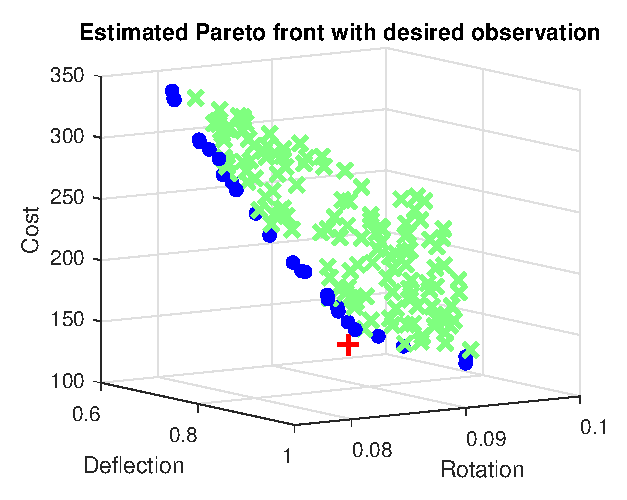
\includegraphics[scale=0.8]{FIG_est_PF_with_des_obs.eps}
%\captionsetup{width=.7\linewidth}
\caption{Each x represents a non-Pareto optimal point drawn from the predictive distribution through preliminary CTO in the wind turbine design application. The dots indicate the estimated Pareto front. The plus sign is the target selected as the performance objective in our proposed design approach.}
\label{fig:elbow}
\end{figure}
%
To do so, we set the point $(\mathrm{deflection}=0.75\mathrm m,\ 
\mathrm{rotation}=0.09\ \mathrm{rad},\ 
\mathrm{cost}=\$130.34)$
 as the target outcome, constant as a function of temperature.
%
Based on the estimated Pareto front, the target outcome is approximately 0.2 units away on the standardized scale.
%
Therefore, we set $\lambda_\delta=1/0.2^2=25.$
%

In the subsequent CTO step, we employed the same MCMC approach as in the preliminary round, except that $\lambda_\delta$ was now fixed.
%
The marginal posterior distribution of the design variables is shown in Figure \ref{fig:wt_marg_post} as contours of highest density regions.
%
The contrast of the posterior distribution with the prior, which is uniform over the area shown in the figure, indicates that strong Bayesian learning has occurred in the design process.
%
%\begin{figure}
%\centering
%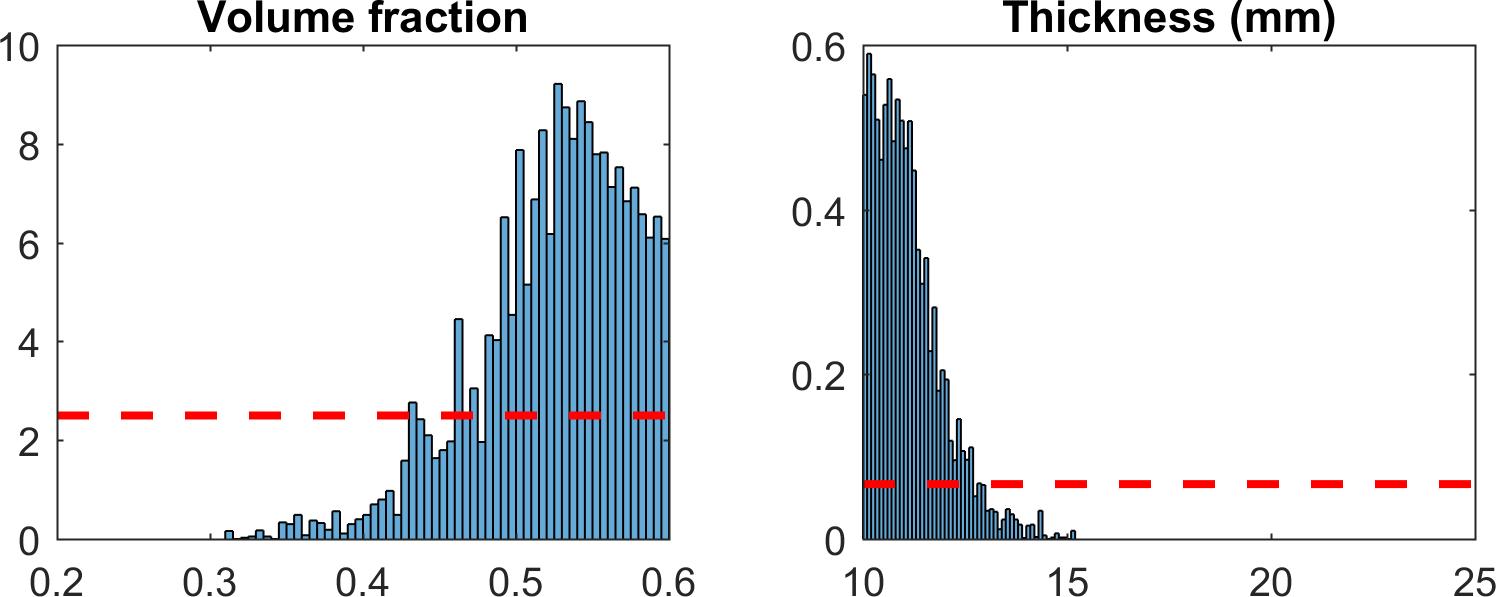
\includegraphics[width=.7\linewidth]{FIG_posterior_marginals_with_priors}
%\captionsetup{width=.7\linewidth}
%\caption{The histograms show the marginal posterior of each calibration parameter. The dotted lines show the priors.}
%\label{fig:wt_marg_post}
%\end{figure}
\begin{figure}
\centering
%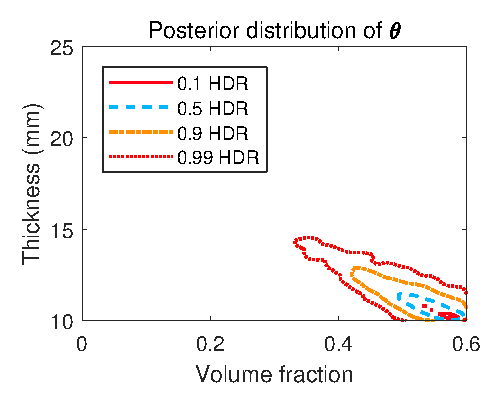
\includegraphics[width=.4\linewidth]{FIG_post_dist_contourplot}
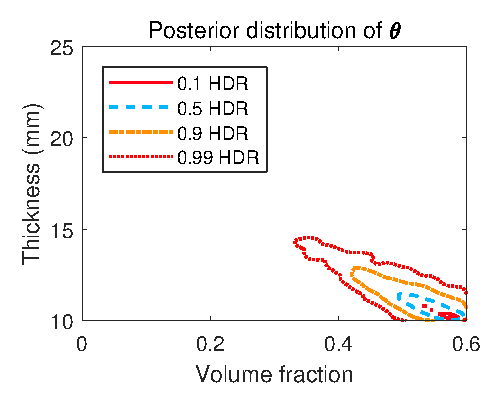
\includegraphics[scale=0.8]{FIG_post_dist_contourplot}
%\captionsetup{width=.7\linewidth}
\caption{Contours of highest density regions of the posterior distribution from CTO in the wind turbine blade system. The prior is uniform over the area shown.}
\label{fig:wt_marg_post}
\end{figure}
%
The prior and posterior marginal predictive distributions of the model outputs are shown in Figure \ref{fig:prior_post_pred_comp}.
%
\begin{figure}
\centering
%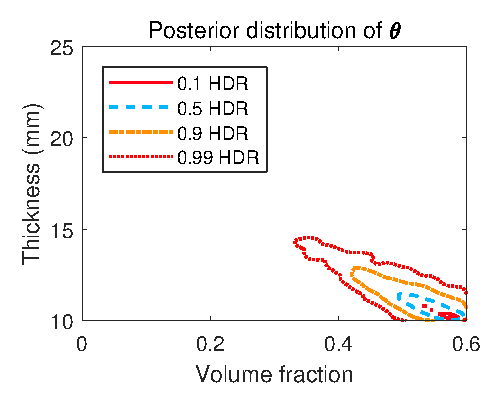
\includegraphics[width=.4\linewidth]{FIG_post_dist_contourplot}
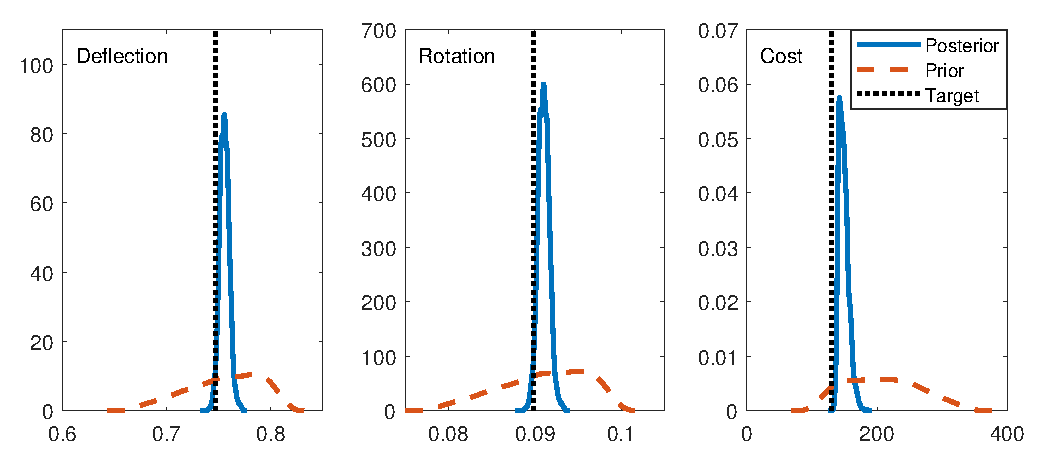
\includegraphics[scale=0.8]{FIG_prior_vs_posterior_dist}
%\captionsetup{width=.7\linewidth}
\caption{Approximate prior and posterior marginal predictive densities for each of the three model outputs. Note that it is to be expected that the posteriors peak near the target (and not on it), since the target was intentionally chosen to lie outside the model range.}
\label{fig:prior_post_pred_comp}
\end{figure}
%
Each marginal posterior density peaks sharply near the target outcome.
%
The mean model output under the prior is $(\text{deflection}=0.76\mathrm m,\ \text{rotation}=0.09\text{ rads},\ \text{cost}=\$207.90/\mathrm m^2)$, whereas under the posterior it is $(0.76\mathrm m,0.09\ \mathrm{rad},\$149.47/\mathrm m^2)$.
%
Though the mean performance outcomes are approximately the same under the posterior distribution as under the prior, the mean cost per square meter and the uncertainty of the outcomes have both been dramatically reduced.
%
If one desires instead to prioritize gains in performance over cost, this can be accomplished by selecting target outcomes that reflect those priorities, as we discuss in Section \ref{removing_cal_pars}. 

\subsection{Pareto front estimation}\label{removing_cal_pars}

%\subsubsection{Motivation}

Often in the case of a system with multivariate output, one might not antecedently have a clear goal for design.
%
All else being equal, when all outputs are to be minimized, any point in the Pareto front is optimal relative to some set of priorities.
%
If those priorities have not been explicitly determined prior to the design process, then no particular outcome can be targeted.
%
In determining one's priorities, it is helpful to know the Pareto front of the relevant system.
%
For example, in a system where quality is monotonically increasing in cost, depending on one's tolerance for high cost, any point in the model range might be optimal.
%
%In determining one's priorities and selecting a target outcome, it is valuable to have a clear and accurate understanding of the Pareto front of the system.
%
In low-dimensional cases, CTO may be used to achieve a holistic picture of the Pareto front by optimizing to each target outcome on a grid.
%
To do this, where the model output is $d-$dimensional, one may draw a grid over the range of $d-1$ of the model outputs and perform CTO to minimize the remaining output at each point of the grid.
%
The $d-1$ outputs, at each grid point, are treated as known up to observation error (meaning that the discrepancy function $\delta(\cdot)$ is set to 0 in the dimension of these outputs).
%
The resulting estimate is distinguished from other methods of estimating the Pareto front (including from the filtering method employed in preliminary CTO) in that it allows for quantifying the uncertainty associated with the Pareto front.
%

Our proposed procedure is illustrated here using the wind turbine blade application.
%
For simplicity, rotation has been removed as a model output, leaving a system with 2-dimensional output of deflection and cost. 
%
The range of cost is known (via preliminary CTO) to be $[\$96,\$352]$.
%
A 20-point grid was drawn over this range of costs. 
%
%Using the rough estimate of the Pareto front from preliminary CDO, we found that to cover the Pareto front, the cost grid should cover the range $[\$96,\$352]$.
%
For each point $c$ in the cost grid, we used the point $(0\mathrm m,\$c)$ as the target outcome for calibration (constant with respect to temperature).
%
For each such point, we then updated this initial target outcome to improve identifiability using the rough estimate of the Pareto front from preliminary CTO using target outcome $(0\mathrm m,\$0)$.
%
Note that only one round of preliminary CTO was needed for this purpose, rather than a separate instance at each grid point.
%

The result of the strategy is to provide an estimate of the response surface with included uncertainty quantification describing, for each point in the grid, the optimal achievable outcome for the output not included in the grid.
%
This enables a decision-maker to visualize the space of desirable possibilities with associated uncertainty metrics. 
%
They can do so without the need for rigorously predetermining their exact priorities for weighing gains in each of the outputs against one another.
%
The result of applying this strategy to the wind turbine blade application is shown in Figure \ref{fig:known_cost}. 
%
\begin{figure}
\centering
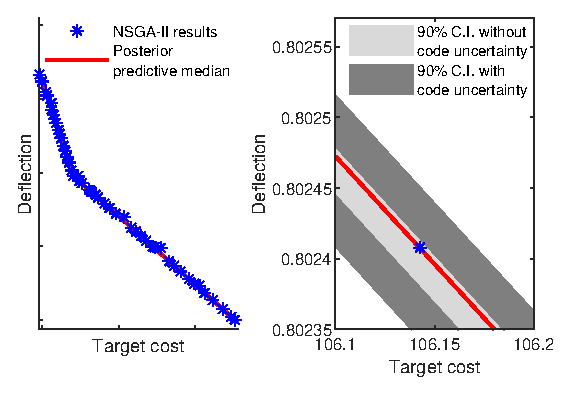
\includegraphics[scale=.8]{FIG_cost_grid_pareto_bands.eps}
%\captionsetup{width=.7\linewidth}
\caption{The lefthand plot shows the posterior predictive distribution of cost as a function of target cost, verifying that the calibration achieved the ``known" costs up to small error. The righthand plot shows the posterior predictive distribution of optimal deflection as a function of target cost, and therefore is an estimate of the Pareto front for the system with attendant uncertainty quantification.}
\label{fig:known_cost}
\end{figure}
%
The lefthand plot shows that the posterior model predictions respected the ``known'' cost values used in the design process.
%
The Pareto front for the system, along with associated uncertainty bands, appears in the righthand plot.
%
This plot visualizes a distribution on the optimal performance outcome for any cost that a decision-maker might select as a budget for production, which would be helpful when selecting a budget.
%
For example, the point of maximum curvature around \$140 manifests itself as a potentially attractive choice, since it can be seen in the plot that prior to that point each dollar spent brings significant gains in reducing deflection.
%
Spending above that level continues to reduce deflection, but less sharply.

The use of CTO in the wind turbine calibration case illustrates how preliminary CTO may be used, not merely to improve the identifiability of a pre-determined optimal region as in Section \ref{example}, but rather to identify a desirable region of the model range and select target outcomes that design to that region.
%
In the wind turbine case, selecting $(0,0,0)$ as one's target determines the optimal region to be the high-cost region toward the upper-left of Figure \ref{fig:elbow}, since (on the standardized scale of model outputs) that region happens to be closest to the target.
%
If one has substantive goals that drive one to select that target, then one is well-served by optimizing to that high-cost region.
%
But if the target $(0,0,0)$ is chosen arbitrarily, then the resulting optimal region is itself determined arbitrarily.
%
The estimate of the Pareto front provided by preliminary CTO allows us to identify regions of special interest, and to select target outcomes that that lead to clearly defined designs, as illustrated in Figure \ref{fig:elbow}.
%
The use of CTO in this case also demonstrates the value of obtaining a posterior distribution on the design variables, rather than just a point estimate.
%
For example, Figure \ref{fig:wt_marg_post} shows not just that a reasonable point estimate of the optimal $\boldsymbol\theta$ is at (.58, 10.2mm), but also that if the volume fraction is lowered to 0.4 it is important to simultaneously raise the thickness to 14mm.
%
More generally, one can see in Figure \ref{fig:wt_marg_post} an indication of the range of $\boldsymbol\theta$ values that achieve results near the target, which is potentially useful when one's goal is to set tolerances (rather than a specific value) for $\boldsymbol\theta$.
%
Finally, the use of CTO in the wind turbine case illustrates how the method can deliver ``Pareto bands'', providing not merely an estimate of the Pareto front (as in preliminary CTO) but also uncertainty associated with that estimate.
%
Such an estimate can be of use to decision-makers when deciding on performance goals subject to budgetary constraints.




\section{Conclusion} \label{conclusion}
% Discussion of the role of computer model validation as a potential methodology for design

We have described how the 
%theoretical background for the use of Gaussian processes to emulate computationally expensive computer model code, and the 
computer model calibration framework established by \cite{Kennedy2001} can be adapted to address questions of engineering design. 
%
Calibration to target outcomes is a modification of that framework which undertakes design by ``calibrating'' a computer model, not to field observations, but rather to artificial data representing performance and cost goals for the system. 
%
The procedure optionally includes a computationally cheap preliminary step that provides a rough estimate of the Pareto front, which may be used to select target outcomes that promote strong Bayesian learning.
%
The resulting posterior predictive distribution is induced to approximate the target outcomes, so that the posterior distribution of $\boldsymbol\theta$ constitutes a distribution on optimal design settings for the system.
%
Repeated applications of this methodology allow one to construct a thorough estimate of the Pareto front of the system with quantified uncertainties.
%
Unlike other methods of Bayesian optimization (a review of which was provided by \citealt{Shahriari2016}), CTO does not require the ability to evaluate model output adaptively.
%
Instead, it can operate using a batch of observations gathered prior to (and independently of) the design process.
%
We described the implementation of this approach in an MCMC routine along with considerations to accommodate computational instability.
%
The use of this methodology is illustrated in the case of material design for a wind turbine blade. 
%
We have shown thereby a variety of ways in which CTO can be used to guide decision-makers in the design process. 
%
By expropriating established tools of model calibration, CTO offers a method of optimization which is sensitive to, and quantifies, all sources of uncertainty.
%

%
The methodology as described here treats the computer model as universally valid over the domain of the design variables. 
%
Future work in this area will include the use of a second discrepancy term capturing model bias.
%
That is, while CTO as presented above includes $\delta(\cdot)$ to capture systematic discrepancy between the target outcomes and the true system, it assumes that the computer model is an unbiased estimate of the true system.
%
The inclusion of a second discrepancy term to capture systematic differences between the model and the observed reality would avoid this idealizing assumption.
%
Other possible extensions of our proposed methodology include its application to so-called ``state-aware calibration'' \citep{Atamturktur2015,Stevens2018,Brown2016}, which would allow the optimal region of the design variables to vary as a function of the control inputs.



\bigskip
\begin{center}
{\large\bf SUPPLEMENTARY MATERIAL}
\end{center}

\begin{description}

%\item[Title:] Brief description. (file type)

\item[\scshape{Matlab} code for CTO:] This includes the example model described in Section \ref{example}, along with code to perform CTO on that system and thereby reproduce Figure \ref{fig:toy_sim_results}.

%\item [{\fontfamily{cmu}\selectfont \sc Testing} code for CDO:] This includes

%\item[R-package for  MYNEW routine:] R-package �MYNEW� containing code to perform the diagnostic methods described in the article. The package also contains all datasets used as examples in the article. (GNU zipped tar file)
%
%\item[HIV data set:] Data set used in the illustration of MYNEW method in Section~ 3.2. (.txt file)

\end{description}

\bibliographystyle{Chicago}

\bibliography{lit_review}
\end{document}

\begin{figure}
\begin{center}
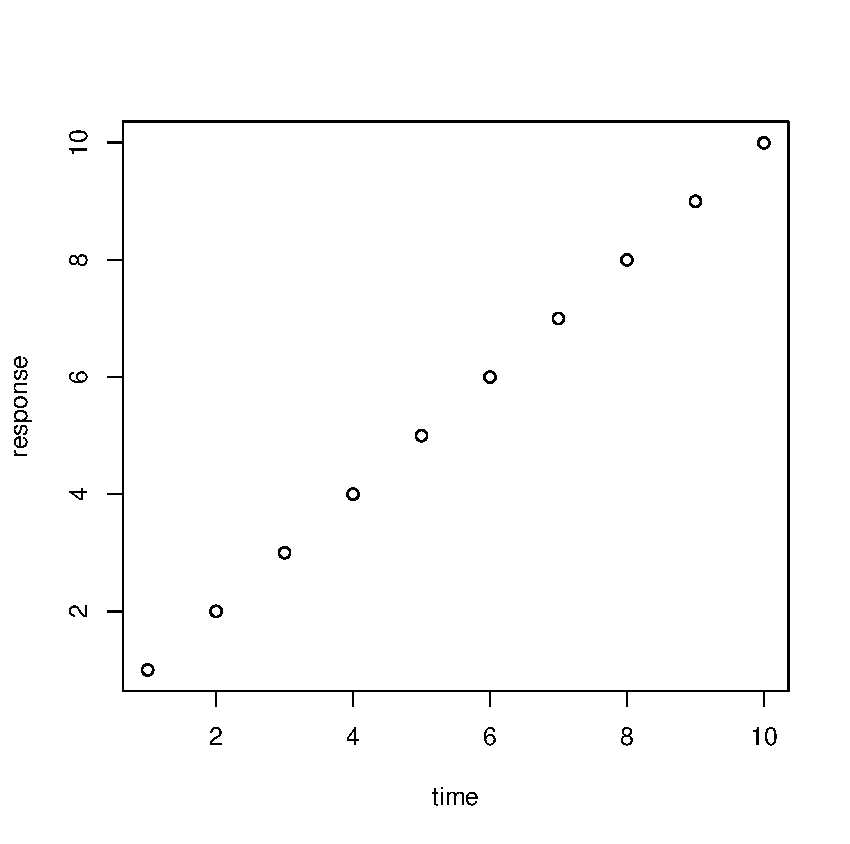
\includegraphics[width=3in]{fig1.pdf}
\end{center}
\caption{Consistency comparison in fitting surrogate model in the tidal
power example. \label{fig:first}}
\end{figure}

\begin{table}
\caption{D-optimality values for design $X$ under five different scenarios.  \label{tab:tabone}}
\begin{center}
\begin{tabular}{rrrrr}
one & two & three & four & five\\\hline
1.23 & 3.45 & 5.00 & 1.21 & 3.41 \\
1.23 & 3.45 & 5.00 & 1.21 & 3.42 \\
1.23 & 3.45 & 5.00 & 1.21 & 3.43 \\
\end{tabular}
\end{center}
\end{table}

\begin{itemize}
\item Note that figures and tables (such as Figure~\ref{fig:first} and
Table~\ref{tab:tabone}) should appear in the paper, not at the end or
in separate files.
\item In the latex source, near the top of the file the command
\verb+\newcommand{\blind}{1}+ can be used to hide the authors and
acknowledgements, producing the required blinded version.
\item Remember that in the blind version, you should not identify authors
indirectly in the text.  That is, don't say ``In Smith et. al.  (2009) we
showed that ...''.  Instead, say ``Smith et. al. (2009) showed that ...''.
\item These points are only intended to remind you of some requirements.
Please refer to the instructions for authors
at \url{http://www.tandfonline.com/action/authorSubmission?journalCode=utch20&page=instructions#.UieFdDafgx0}
\item If you have Supplementary Material (eg software, data, technical
proofs), identify them in the section below.  In early stages of the
submission process, you may be unsure what to include as supplementary
material.  Don't worry---this is something that can be worked out at later stages.
\end{itemize}
